% !TeX spellcheck = en_GB

\section{The Neural Engineering Framework}
\label{sec:nef}

\begin{figure}[p]
	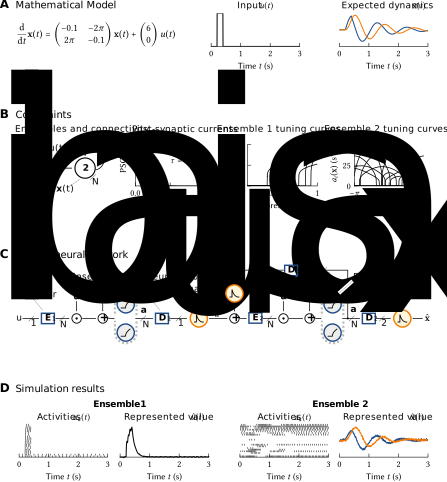
\includegraphics{media/chapters/02_modelling/02_03/nef_overview.pdf}
	\caption[Overview of the Neural Engineering Framework]{Overview of the Neural Engineering Framework (\NEF).
	\textbf{(A,~B)} Researchers provide a mathematical model or sampled data (sampled data shown here are random and only for illustration purposes), as well as a set of constraints.
	In this example, constraints are the overall connectivity, tuning properties and filter properties of post-synaptic currents. $\angle \vec x$ denotes the angle of $\vec x = (x_1, x_2)$, i.e., $\angle \vec x = \mathrm{arctan2}(x_2, x_1)$. \textbf{(C)} The \NEF can be used to systematically construct a spiking neural network from the given data. This network optimally implements the mathematical model under the given constraints.
	\textbf{(D)} Simulating the network gives insights into how well the mathematical description can be implemented on a neural substrate.
	Spike raster plots with neural activity depict output spikes (short vertical lines) for each neuron (corresponding to rows) over time.}
	\label{fig:nef_overview}
\end{figure}

As we mentioned at the beginning of this chapter, the Neural Engineering Framework (\NEF; \cite{eliasmith2003neural}) is a modelling framework for neurobiological systems.
The \NEF combines techniques from engineering and mathematics---particularly control and dynamical systems theory---with the neurobiological concepts discussed before.
The goal is to allow researchers to map high-level descriptions of cognitive phenomena onto low-level spiking neural networks.
As such, the \NEF provides a synthesis of bottom-up and top-down modelling, and is an attempt at a theory of neuroscience that spans multiple levels of analysis.

To use the \NEF, researchers systematically apply three \enquote{principles} that encapsulate key assumptions about neurobiological systems.
These principles exploit neural nonlinearities and synaptic filters to describe how vectorial quantities can be represented, transformed, and made to follow certain dynamics in a spiking neural fabric.
The resulting neural networks adhere to mechanistic constraints, such as neural connectivity, maximum firing rates, tuning properties, and synaptic time-constants.
This is illustrated schematically in \Cref{fig:nef_overview}.
A software tool that automates the process of translating mathematical models into spiking neural networks using the \NEF principles is part of the Nengo spiking neural network simulator package \citep{bekolay2014nengo}.\footnote{See \url{https://www.nengo.ai/} for more information on Nengo. Nengo is free for non-commercial use.}


%\begin{enumerate}[1.]
%	\item \emph{Representation.}
%	The momentary activity $\vec a \in \mathbb{R}^{\Npop}$ of an ensemble of \Npop neurons represents a vectorial quantity $\vec x \in \mathbb{R}^d$. The encoding process mapping $\vec x$ onto activities $\vec a$ is nonlinear,
%	the decoding process is linear.
%	That is, there exists a matrix $\Dec \in \mathbb{R}^{d \times \Npop}$ such that $\vec x \approx \vec \Dec \vec a(\vec x)$.
%	\item \emph{Transformation.}
%	Synaptic connections between neural ensembles approximate nonlinear transformations $f(\vec x)$ applied to the represented values, where $f : \mathbb{R}^d \longrightarrow \mathbb{R}^{d'}$ and $d$ and $d'$ are the dimensionalities of the quantities represented in the individual ensembles.
%	\item \emph{Dynamics.}
%	Represented values are state variables $\vec x(t)$ in a dynamical system. Recurrent connections approximate arbitrary dynamical systems of the form $\dot{\vec x} = f(\vec x(t), \vec u(t), t)$.
%	Here, $\vec x(t)$ is the represented value, $\vec u(t)$ is some external input, and $t$ is the current time.
%\end{enumerate}

In this section, we first discuss applications of the \NEF from the perspective of the cognitive sciences (model validation and hypothesis generation), as well as engineering and computer science (a programming model for neuromorphics).
We continue with a detailed description of the theory underpinning the \NEF, and conclude with a list of limitations that we address in the next chapters.

\subsection{Model Validation and Hypothesis Generation}
\label{sec:nef_purpose}

As we alluded to in the introduction of this chapter, models built using the \NEF bridge multiple levels of analysis.
That is, they implement high-level behaviour (given as a mathematical description) using low-level mechanisms (spiking neurons and synapses).
This facilitates model validation and hypothesis generation.

\subsubsection{Model validation}
The concept of model validation generally refers to comparing a model to empirical measurements \citep{adams2012assessing}.
In the case of \NEF models, we can, of course, compare the high-level behaviour of the biological system to that of the constrained network model.
The smaller the deviations, the \enquote{better} the original mathematical model.%
\footnote{Of course, naively evaluating models in this manner does not account for overfitting. The model could inadvertently be tuned to reproduce the behaviour of interest, but not be able to generalise to different scenarios. In contrast to other machine learning approaches, overfitting in this sense is typically less of a problem with \NEF models.
This is due to the transparency of the training process, only few (typically hand-selected) parameters, and biological constraints, all of which can be seen as regularisation.}
While such comparisons would also be possible with the high-level model alone, biological constraints can drastically influence the high-level behaviour of the model.
The \NEF is thus a good litmus test for the suitability of a mathematical model to be realised on a neural substrate.
This is because the \NEF \emph{optimally} implements a set of mathematical equations as an idealised spiking neural network.
If the model cannot be realised on a spiking neural substrate despite these idealised conditions, it is unlikely that it describes a biological process well.

\NEF models can also be compared in terms of detailed neurophysiological data, and not just high-level behaviour.
Because \NEF models are based on a biologically plausible neural substrate, researchers can measure neurophysiological quantities, such as spike trains, local field potentials, or blood oxy\-gen\-ation \citep[Chapters 5.8~\&~9.4]{eliasmith2013how}.
Examples of this can be found in \citet{stewart2012learning,bekolay2014spiking,duggins2017effects,voelker2018improving,gosmann2021cue}.

\subsubsection{Hypothesis generation}
There are two ways in which the \NEF aids \emph{hypothesis generation}.
First, and closely related to model validation, deviations between the constrained simulation and the original mathematical model may indicate that the high-level description cannot be realised by the biological system.
Hence, the \NEF can be used to reject unsuitable hypotheses and to guide theories towards higher degrees of biological plausibility.
Examples of cognitive theories developed in conjunction with the \NEF include the Semantic Pointer Architecture (SPA; \cite{eliasmith2013how}) and SPAUN (the \enquote{Semantic Pointer Architecture Unified Network}), a functional brain model capable of a variety of cognitive tasks \citep{eliasmith2012largescale}.

Second, \NEF models can be used to predict the behaviour of a system in experimental paradigms for which no empirical data exists (yet).
This prediction then forms a hypothesis that can be compared to future empirical data.
Furthermore, the \NEF also enables the systematic variation of observed biological parameters (e.g., time-constants or connectivity), which is often not easily possible in real biological systems.
Assessing the system performance in such artificial situations may yield hypotheses as for why evolution favoured certain parameter combinations.
We give an example of this in \Cref{chp:cerebellum}.

\subsection{Applications to Neuromorphic Computing}
\label{sec:neuromorphic}

The scientific applications discussed above were the primary motivation for the development of the \NEF.
However, coincidentally, the same methods are useful as a programming model for neuromorphic computers \citep{boahen2017neuromorph,voelker2021programming}.

\subsubsection{Neuromorphic computers}
Coined by \citet{mead1990neuromorphic}, this term refers to computer systems that---to some degree---mimic information processing in the brain.
This typically implies numerous simple computational units, \emph{neurons}, connected via a flexible interconnect \citep{furber2016largescale}.
Beyond these basic characteristics there is no consensus as for what exactly constitutes a \enquote{neuromorphic computer}.
However, most neuromorphic hardware systems execute computations asynchronously and possess provisions for sparse event-based signalling.
Akin to biology, individual computational units independently generate binary events.
In contrast to artificial neural networks, computation is inherently temporal; communication occurs sporadically and does not carry continuous values.
Hence, the underlying communication infrastructure solely carries temporally sparse spike events, minimising the amount of transferred data.

Current neuromorphic computers can be roughly split into two categories, depending on the specific realisation of the computing elements.
Computation either takes place in analogue model circuits, similar to the \LIF circuit (\Cref{fig:lif}), or digital processors with varying degrees of programmability.
Examples of systems in the former \enquote{mixed-signal} category include Braindrop \citep{neckar2019braindrop} and BrainScaleS \citep{schemmel2010waferscale}.
Systems that fall into the latter \enquote{purely digital} category are SpiNNaker \citep{furber2013overview} and Loihi \citep{davies2018loihi}. See \citet{furber2016largescale} for a more comprehensive list.

\subsubsection{Applications of neuromorphic computing}
The primary motivation behind neuromorphic hardware is to construct computing hardware that approaches the energy efficiency of biological brains \citep{mead1990neuromorphic,boahen2017neuromorph}.
Compared to conventional computer architectures, these energy savings are mostly due to the asynchronous nature of the computational units, as well as the reduction in communication bandwidth due to event-based signalling \citep{painkras2013spinnaker}.
Furthermore, mixed-signal neuromorphic computers with analogue model circuits benefit from each computational unit operating close to the theoretically required minimum energy \citep{boahen2017neuromorph}.
However, compared to purely digital systems, such analogue designs are much more challenging to build from an engineering perspective.

Being able to reliably simulate large spiking neural networks with a low energy footprint would be a major scientific breakthrough.
For example, this would enable large-scale brain simulations that are infeasible with conventional supercomputers \citep{calimera2013human}.
From an engineering perspective, being able to map artificial neural networks onto neuromorphic computers could greatly reduce energy costs of machine learning in the data centre and enable new mobile applications of artificial intelligence \citep{hunsberger2016training,blouw2018benchmarking,goltz2021fast,blouw2020eventdriven}.
Due to the inherent temporal aspect of the computation, spiking neural networks and neuromorphic hardware are particularly well-suited for applications requiring real-time stream processing, such as robotic control or autonomous drones \citep{komer2015biologically,yan2021comparing}.

\subsubsection{The \NEF as a programming model for neuromorphic computers}
While, as of writing, several neuromorphic hardware platforms are available to the wider research community, a remaining challenge is to actually program these systems.
Since the computational fabric of neuromorphic computers is similar to biological neural substrates, the \NEF can be used to translate mathematical descriptions of dynamical systems into network models that can be executed on the hardware system \citep{boahen2017neuromorph}.
The given constraints can be used to reflect the capabilities of the hardware and to specify the desired precision of the computation.
A variety of neuromorphic platforms have been included as an execution target in Nengo, catering to both scientific and engineering applications.

\pagebreak

\subsection{Principle 1: Representation}

\label{sec:nef_representation}

As we saw above, the Neural Engineering Framework has useful applications in both science and engineering.
In the first part of this thesis, we discuss extensions to the \NEF that allow us to model neurobiological circuits more accurately and to take better advantage of the computational resources found on neuromorphic computers.
In preparation for these extensions, we now provide a detailed discussion of the aforementioned \enquote{three principles} at the core of the \NEF.

The first two \NEF principles are best explained assuming steady-state average activities, although, as mentioned before, biological neural networks inherently form dynamical systems.
However, our use of average rate approximations should not be interpreted as the adoption of a \enquote{rate code} by the \NEF, but, as we discuss below, is a convenience for solving the synaptic weight optimisation problem.
All optimisations can be done in the spiking domain, but the computational costs are significantly higher~\citep{macneil2011finetuning}.

For now, our goal is to map static equations of the form $\vec y = f(\vec x)$ onto rate approximations of spiking neural networks.
The first \NEF principle describes how neuron populations represent quantities such as $\vec x$ and $\vec y$.
Paraphrasing \citet{eliasmith2003neural}:
\begin{framed}
\noindent\emph{\NEF Principle 1.}
The momentary activity $\vec a \in \mathbb{R}^{\Npop}$ of a population of \Npop neurons represents a vectorial quantity $\vec x \in \mathbb{R}^d$. The encoding process mapping $\vec x$ onto activities $\vec a$ is nonlinear,	the decoding process is linear.
That is, there exists a matrix $\Dec \in \mathbb{R}^{d \times \Npop}$ such that $\vec x \approx \vec \Dec \vec a(\vec x)$.
\end{framed}
There are two fundamental assumptions in this principle that deserve to be untangled.
First, we assume that neuron \emph{populations} form basic functional units and, second, that biological systems represent vectorial quantities.
We already discussed the first assumption regarding populations in more detail in \Cref{sec:neural_tuning}.
To summarise, neighbouring neurons are sensitive to the same quantity and neural activities are noisy---this suggests that nervous systems use population codes.
The second assumption deserves more explanation, given that vectors are abstract mathematical objects.

\subsubsection{Vectorial representations}
The assumption that populations represent vectors $\vec x \in \mathbb{R}^d$ is---to some degree---a mathematical convenience.
Many mathematical objects have useful equivalent vectorial representations, including functions \citep[Chapter 3]{eliasmith2003neural}, probability densities \citep[Chapter 9]{eliasmith2003neural}, and symbols (via vector symbolic architectures; see \cite{gayler2003vector}, \cite{eliasmith2012largescale} and \cite{eliasmith2013how}).
% TODO: Reference review of function spaces

Additionally, there is strong evidence that the activities of neural populations form smooth low-dimensional manifolds in a high-dimensional activity space \citep{gallego2017neural,stringer2019highdimensional}.
There exists a mapping $\vec a: \mathbb{R}^d \longrightarrow \mathbb{R}^{\Npop}$ (with $d \ll \Npop$) between a low-dimensional vector $\vec x \in \mathbb{R}^d$ and the average neural activities $\vec a(\vec x) \in \mathbb{R}^{\Npop}$, where \Npop is the number of neurons in the population.
If the population exhibits activities $\vec a(\vec x)$ associated with a value $\vec x$, then the population \emph{represents} a \Ndim-dimensional quantity $\vec x$.

\subsubsection{Encoding vectorial quantities}

\begin{figure}
	\centering
	\includegraphics{media/chapters/02_modelling/02_03/nef_representation_2d.pdf}
	{\phantomsubcaption\label{fig:nef_representation_2d_surface}}
	{\phantomsubcaption\label{fig:nef_representation_2d_unit_circle}}
	\caption[Obtaining bell-shaped tuning curves when using two-dimensional encoders]{Obtaining bell-shaped tuning curves when using two-dimensional encoders. Figure adapted from \citet[Figure~2.8, p.~52]{eliasmith2003neural}.
	\textbf{(A)} The surface plot of the tuning curve of a single neuron. The orange arrow points in the direction of the encoder $\vec e_i$.
	\textbf{(B)} The tuning curve for a represented value $\vec x$ of constant magnitude over the angle $\angle \vec x$.
	The orange triangle corresponds to the direction of the encoder.
	The neuron is most active for represented values pointing in this direction.
	}
	\label{fig:nef_representation_2d}
\end{figure}

As we have discussed in \Cref{sec:neural_tuning}, the relationship between a stimulus $\vec x$ and activities of an individual neuron are also referred to as a \enquote{tuning curve}.
While tuning curves in neuroscience are typically defined over scalar quantities, \citeauthor{eliasmith2003neural} propose a parametrised encoding equation $a_i(\vec x)$ that maps $\vec x \in \mathbb{R}^{\Ndim}$ onto the activities of the $i$th neuron in a population---similar to the mathematical model we presented to describe tuning curves in the Hubel and Wiesel experiment (\Cref{sec:neural_tuning},  \Cref{fig:visual_cortex_receptive_field_example} and eq.~\ref{eqn:tuning_curve_from_receptive_field}):
\begin{align}
a_i(\vec x) = G\big[J_i\big(\langle \vec x, \vec e_i \rangle\big)\big] = G\big[\alpha_i\langle \vec x, \vec e_i \rangle + \beta_i\big] \,,
 \quad\quad \text{where } i \in \{1, \ldots, N\} \,.\label{eqn:encoding}
\end{align}
Depending on the interpretation, the encoding vector $\vec e_i$ is equivalent to the \enquote{receptive field} or \enquote{preferred direction} of the neuron.
For example, as depicted in \Cref{fig:nef_representation_2d}, a two-dimensional encoding vector can be used to construct bell-shaped tuning curves similar to those discussed in the context of orientation tuning in the visual cortex; here, the vector $\vec e_i$ would stand for a preferred direction.
Of course, $\vec e_i$ and $\vec x$ could also be discretised visual stimuli---in this case, $\vec e_i$ would be a receptive field and \cref{eqn:encoding} is a discrete approximation of \cref{eqn:tuning_curve_from_receptive_field}.

The response curve $G[J]$ depends on the underlying neuron model; for example, we derived the response curve for \LIF neurons in \Cref{sec:simplified_neuron_models} (eq.~\ref{eqn:lif_response_curve}); 
the current translation function $J_i(\xi)$ is typically an affine mapping parametrised by a gain $\alpha_i$ and a bias current $\beta_i$.

When building \NEF systems, modellers choose the parameters of $a_i(\vec x)$ to characterise how a stimulus $\vec x$ \emph{should} be reflected in the activities of individual neurons.
This last emphasis on \emph{should} is important.
Modellers establish a \emph{normative constraint}.
They specify what the desired tuning should \emph{optimally} be---for example, taking biological data into account.
The purpose of the \NEF is to ensure that this constraint is met in a network context.


\begin{figure}
	\centering
	\hspace{-0.2cm}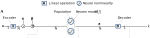
\includegraphics{media/chapters/02_modelling/02_03/nef_representation_diagram.pdf}
	\includegraphics{media/chapters/02_modelling/02_03/nef_representation.pdf}
	{\phantomsubcaption\label{fig:nef_representation_diagram}}
	{\phantomsubcaption\label{fig:nef_representation_current_translation}}
	{\phantomsubcaption\label{fig:nef_representation_tuning_curves}}
	{\phantomsubcaption\label{fig:nef_representation_deocding}}
	\caption[Representation in the Neural Engineering Framework]{Representation in the Neural Engineering Framework. Example for a population of $N = 10$ neurons representing a one-dimensional quantity.
	\textbf{(A)} Schematic overview of the encoding and decoding process.
	\textbf{(B)} Randomly selected affine current translation functions $J_i(\xi) = \alpha_i \langle \vec x, \vec e_i \rangle + J^\mathrm{bias}_i$. The dotted line corresponds to the activity threshold $J_\mathrm{th}$.
	\textbf{(C)} Tuning curves for each neuron in the population after applying the somatic nonlinearity $G[J]$~(eq.~\ref{eqn:lif_response_curve}).
	\textbf{(D)} Reconstructing the represented value from neuron activity by means of linear decoding. Dashed line corresponds to the ideal.}
	\label{fig:nef_representation}
\end{figure}

\subsubsection{Selecting encoders, gains, and biases}
Of course, this raises the question of how modellers should select encoders $\vec e_i$, biases $\beta_i$, and gains $\alpha_i$.
To form a good basis for a population code, the population must exhibit diverse tuning (cf.~\Cref{fig:population_code}).
At the same time, the tuning curves must stay within modelling constraints such as the maximally observed firing rates $a_i$ for the range of stimuli $\vec x$ over which we characterise the neuron population.
We denote the set of represented values as a compact set \Xrepr with finite, non-zero volume $\vol(\Xrepr)$.

Unless more specific data are available, we can for example assume that $\vec x$ are within a hyperball of radius $r$, i.e., $\Xrepr = r \Ball^d$.
The encoding vectors $\vec e_i$ can be sampled from the unit hypersphere $\mathbb{S}^d$.
For monotone increasing response curves $G$, gain $\alpha$ and bias $\beta$ can be computed for each neuron by sampling an \enquote{$x$-intercept} value $\xi_0$ from the interval $[-r, r]$ and a maximum rate $a_\mathrm{max}$.
We then solve for $\alpha$, $\beta$ such that the following equations hold:
\begin{align*}
	\alpha \xi_0 + \beta &= J_0 = G^{-1}[0] \,, &
	\alpha r + \beta &= J_\mathrm{max} = G^{-1}[a_\mathrm{max}] \,, & \text{where } G^{-1}[a] &\coloneqq \max \big\{ J \mid G[J] = a \big\} \,.
\end{align*}
We get $(r - \xi_0) \alpha = J_\mathrm{max} - J_0$, $(r - \xi_0) \beta = (r J_0 - \xi_0 J_\mathrm{max})$.
For example, for each tuning curve in \Cref{fig:nef_representation}, we randomly sampled a $\xi_0$ from a uniform distribution over $[-1, 1]$, and a maximum firing $a_\mathrm{max}$ rate uniformly from $[10, 50]$.

\subsubsection{Computing identity decoders}
\Cref{eqn:encoding} describes the average neural activities $\vec a$ we expect when a population is representing a certain value $\vec x$; that is, this equation describes how quantities $\vec x$ are \emph{encoded} in a neural network.
Complementary to encoding is \emph{decoding}.
That is, given the activities $\vec a$, we would like to reconstruct the represented $\vec x$.
This could---for example---be accomplished using Bayesian inference, as we demonstrated in \Cref{fig:population_code}.
If the number of neurons \Npop in a population is large enough we can, to a very similar effect, just use a linear decoding matrix \Dec (\Cref{fig:nef_representation}; \cite{salinas1994vector}).

The idea is to simply multiply the activities $\vec a$ with a matrix $\Dec \in \mathbb{R}^{d \times \Npop}$ such that the decoded $\vec{\hat x} = \Dec \vec a(\vec x)$ is approximately equal to the encoded $\vec x$, for any $\vec x \in \Xrepr$.
Under the assumption that the activities $\vec a$ are subject to independent and identically distributed (i.i.d.) zero-mean Gaussian noise with standard-deviation $\sigma$, the decoding matrix \Dec can be obtained by minimising a least-squares loss-function $E$:
\begin{align}
	E &= \frac{1}{\vol(\Xrepr)} \iint_{\Xrepr} \bigl\| \vec x - \Dec \bigl( \vec a(\vec x) + \nu \bigr) \bigr\|_2^2  \, \mathrm{d}\vec{x} \quad\quad \text{where } \nu \sim \Normal(0, \sigma) \,.
	\label{eqn:lstsq_loss_identity}
\end{align}
Of course, minimising this integral directly is infeasible.
We approximate a solution numerically by drawing \Nsmpls samples from \Xrepr, denoted $\vec x_1$, $\ldots$, $\vec x_N$.
Arranging the samples and the corresponding population activities in matrices $\mat X = \begin{pmatrix} \vec x_1, \ldots, \vec x_{\Nsmpls} \end{pmatrix} \in \mathbb{R}^{\Nsmpls \times \Ndim}$ and $\mat A = \begin{pmatrix}\vec a(\vec x_1), \ldots, \vec a(\vec x_{\Nsmpls})\end{pmatrix} \in \mathbb{R}^{\Nsmpls \times \Npop}$, we can phrase finding \Dec as a Tikhonov regularised least-squares optimisation problem
\begin{align}
\min_{\Dec} \sum_{k = 1}^{\Nsmpls} \| \Dec \vec a(\vec x_k) - \vec x_k \|_2^2  + \| \sigma \Dec \|^2_\mathrm{F}
&= \min_{\Dec} \| \mat A \Dec^T - \mat X \|_\mathrm{F}^2 + \sigma^2 \Nsmpls \| \Dec \|_\mathrm{F}^2 \,,
\label{eqn:lstsq_loss}
\end{align}
where $\lambda = N \sigma^2$ is the regularisation factor.
From a probabilistic perspective, this particular choice of $\lambda$ results in the exact maximum a-posteriori solution for $\mat D$ with the prior assumption that there is Gaussian noise with standard deviation $\sigma$ on the measurements $\mat A$ \citep[Chapter~6]{boyd2004convex}. 
Larger $\lambda$ increase the robustness of the solution with respect to noise, but decrease the noise-free approximation error.
The solution can be expressed in terms of the regularised Moore-Penrose pseudo-inverse:
\begin{align}
\Dec^T &= \mat A^+ \mat X \,, &\text{where} \quad \mat A^+ &= \bigl(\mat A^T \mat A + \lambda N \mat I \bigr)^{-1} \mat A^T \,.
\label{eqn:decoding}
\end{align}
As explored by \citet[Chapter~2]{eliasmith2003neural}, the decoding error $E$ tends to decrease with $\mathcal{O}(\sqrt{n})$, assuming that the tuning curves have uniform $x$-intercepts and random encoders $\vec e_i$.
An example of this decoding scheme is given in \Cref{fig:nef_representation_deocding}.

Note that, as mentioned before, we do not take dynamics into account when computing the decoders \Dec.
However, as we discuss next, the same \Dec can be used to decode represented values through time in spiking networks when defining activity $\vec a(t)$ as low-pass filtered population spike trains.
We explicitly take temporal aspects of neural computation into account in \Cref{sec:nef_dynamics} below, and when we discuss temporal tuning in Chapter~4.

\pagebreak

\subsection{Principle 2: Transformation}
\label{sec:nef_transformation}

The representation principle maps vectors $\vec x$ onto average neural activities $\vec a(\vec x)$.
Of course, individual neuron populations seldom exist in isolation.
To construct \emph{networks} that realise the desired tuning properties, we need to determine synaptic weights $w_{ij}$ that describe the connection strength between the $j$th pre- and the $i$th post-neuron.
In addition to realising the chosen representations, the \NEF puts a further modelling constraint on the synaptic weights:
\begin{framed}
\noindent\emph{\NEF Principle 2.} Synaptic connections between neural ensembles approximate nonlinear transformations $\vec y = f(\vec x)$, where $\vec x \in \mathbb{R}^d$ is the value represented in the pre-population, and $\vec y \in \mathbb{R}^{d'}$ the value represented in the post-population.
\end{framed}

\begin{figure}
	\centering
	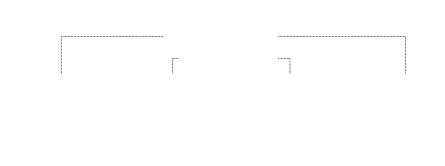
\includegraphics{media/chapters/02_modelling/02_03/nef_transformation_annotations.pdf}%
	\kern-157.19mm\includegraphics{media/chapters/02_modelling/02_03/nef_transformation.pdf}
	\caption[Examples of the function decoding scheme]{Examples of the function decoding scheme. Instead of decoding the represented value $\vec x$ from a neuron population, we can approximate arbitrary functions $f(\vec x)$.
	\textbf{(A)} $\Npop = 20$ tuning curves $\vec a(x)$; same parameters as in \Cref{sec:nef_representation}. \textbf{(B-E)} Different linear decodings $\mat D^f \vec a(x)$ of the above tuning curves. Dotted line is the target function, thick line the decoded function. Inset $E$ is the \RMSE.
	}
	\label{fig:nef_transformation}
\end{figure}

That is, modellers can choose a transformation $f$ that should be computed in a connection.
We can easily approximate functions $f$ of the value $\vec x$ represented in a pre-population using a \emph{function decoder} $\Dec^f$.
This $\Dec^f$ has the property that $\Dec^f \vec a(\vec x) = \vec{\hat y} \approx \vec{y} = f(x)$.
Modifying the least-squares loss from \cref{eqn:lstsq_loss_identity}, we get
\begin{align}
	E &= \frac{1}{\vol(\Xrepr)} \iint_{\Xrepr} \bigl\| f(\vec x) - \Dec \bigl( \vec a(\vec x) + \nu \bigr) \bigr\|_2^2  \, \mathrm{d}\vec{x} \quad\quad \text{where } \nu \sim \Normal(0, \sigma) \,.
	\label{eqn:lstsq_loss_f}
\end{align}
Analogously to the above, a discrete approximation of $\mat D^f$ for \Nsmpls samples ${\vec x}_1$, $\ldots$, ${\vec x}_{\Nsmpls}$ is given as 
\begin{align*}
	\bigl(\Dec^f\bigr)^T &= \mat A^+ \mat Y \,, &\text{where } \mat A &= \begin{pmatrix}\vec a(\vec x_1), \ldots, \vec a(\vec x_{\Nsmpls})\end{pmatrix} \in \mathbb{R}^{\Nsmpls \times \Npop} \,, & \mat Y &= \begin{pmatrix}f(\vec x_1), \ldots, f(\vec x_{\Nsmpls})\end{pmatrix} \in \mathbb{R}^{\Nsmpls \times \Ndim'} \,.
\end{align*}
Examples of functions decoded from $\vec a(\vec x)$ are depicted in \Cref{fig:nef_transformation}.
The decoding error $E$ depends on the number of pre-neurons \Npop, as well as the \enquote{smoothness} of the decoded function.

\begin{figure}
	\centering
	\vspace{0.25mm}
	\includegraphics{media/chapters/02_modelling/02_03/nef_transformation_diagram.pdf}
	\caption[Neuron populations in the NEF as a single-hidden-layer artificial neural network]{Neuron populations in the \NEF form a single-hidden-layer artificial neural network. Encoders $\mat E$, gains $\vec \alpha$, and gains $\vec \beta$ correspond to a fixed input transformation. The function decoder $\Dec^f$ forms a set of linear output weights. Since the input transformations are fixed, computing $\Dec^f$ is simple.}
	\label{fig:nef_transformation_diagram}
\end{figure}

\subsubsection{Comparison to artificial neural networks}
From the perspective of artificial neural networks, the \NEF characterises neuron populations as a single-hidden-layer neural network with a fixed input transformation defined by the encoders, gains, and biases.
Since the input transformation up to the neural nonlinearity---approximated by the response curve $G[J]$---is fixed, learning the output weights---the function decoder---is a convex optimisation problem and no stochastic optimisation such as gradient descent is required (\Cref{fig:nef_transformation_diagram}).

Similar nonlinear encoding and linear decoding schemes have been explored in machine learning for decades.
One early example are the radial basis function networks described by \citet{broomhead1988radial}.
Going back even further, the overall idea is similar to the pattern-recognition model of granule cell activity in the cerebellum proposed by \citet{marr1969theory}.
From a more theoretical perspective, neuron population tuning-curves $\vec a(\vec x)$ span a function space with a set of non-orthogonal basis functions. 
\citet{hornik1989multilayer} show that---assuming a reasonable distribution of these basis functions---we can approximate any continuous function over \Xrepr to a desired degree by increasing the number of hidden units.
% TODO: Reference to other basis function related stuff

\subsubsection{Computing synaptic weights}
As we have seen, function decoders $\Dec^f$ can approximate arbitrary functions $f$ over \Xrepr.
Of course, this is only half of what we set out to accomplish.
Our goal was to find synaptic weights $\mat W \in \mathbb{R}^{m \times n}$ that connect from a pre-population of \Npop neurons representing $\vec x$ to a post-population of $m$ neurons, such that the tuning properties of the target population are preserved, \emph{and} the post-population is representing a transformed version $f(\vec x)$.

If we assume that the current translation function $J_i(x)$ is an intrinsic part of each post-neuron $i$, encoding and decoding can be linearly combined into a weight vector $\vec w_i$:
\begin{align}
	a_i^\mathrm{post}\bigl(f(\vec x)\bigr)
		&\approx
	a_i^\mathrm{post}\bigl(\mat D^f \vec a_\mathrm{pre}(\vec x)\bigr)
		=	
	G\bigl[J_i\bigl(\langle \vec e_i^T, \mat D^f \vec a^\mathrm{pre}(\vec x)\rangle \bigr)\bigr]
		=
	G\bigl[J_i\bigl(\langle \vec w_i, \vec a^\mathrm{pre}(\vec x) \rangle \bigr)\bigr] \,.
	\label{eqn:nef_weight_vector}
\end{align}
Hence, $\mat W = \mat E \mat D^f$ forms a synaptic weight matrix, where $\mat E \in \mathbb{R}^{m \times d'}$ is a matrix of post-population encoding vectors $\vec e_i$, and $\mat D^f$ is the pre-population function decoder.
This matrix implicitly decodes $\vec{\hat y} = f(\vec x)$ from a pre-population, and re-encodes $\vec{\hat y}$ in the post-population.

%Note that these synaptic weights directly translate the pre-population activities into an average current that is injected into the post-neuron.
%Although biological neural networks do not possess \enquote{encoding} and \enquote{decoding} matrices with intermediate low-dimensional representations, the product $\mat W = \mat E \Dec^f$ has the equivalent effect of first decoding, and then re-encoding.

A welcome side-effect of this formalisation is that the weight matrix $\mat W$ is of low rank.
This significantly reduces the amount of computation required to evaluate \NEF networks.
Consider a matrix-vector product of the form $\mat W \vec a$.
Evaluating this requires $\mathcal{O}(mn)$ operations, where \Npop and $m$ are the number of neurons in the pre- and post-population.
In contrast, multiplying the low-rank factorisation with an activity vector, i.e., computing $\mat E ( \mat D \vec a 
)$, requires only $\mathcal{O}(\Ndim n + \Ndim' m)$ operations.
Since, typically, $d \ll n$ and $d' \ll m$, this is a linear time operation.
Along with the linearity of homogeneous synaptic filters, this enables Nengo to simulate large spiking neural networks on commodity hardware \citep{bekolay2014nengo}.

\subsection{Principle 3: Dynamics}
\label{sec:nef_dynamics}

% TODO: Mention the key-word recurrent somwhere!

\begin{figure}
	\centering
	\includegraphics{media/chapters/02_modelling/02_03/instantaneous_spike_rate.pdf}%
	{\phantomsubcaption\label{fig:instantaneous_spike_rate_a}}%
	{\phantomsubcaption\label{fig:first_order_low_pass}}%
	\caption[Estimating the instantaneous firing rate using a synaptic filter]{Estimating the instantaneous firing rate using a first-order exponential synaptic filter. \textbf{(A)} Blue line depicts a spike train (short black lines at the bottom) filtered by a first-order exponential low-pass filter $h(t)$ with $\tau = \SI{0.1}{\second}$. The black line is the \enquote{ground-truth} rate underlying the spike train (using a $\Delta\Sigma$-modulator).
	Apart from a phase shift and some added noise, the low-pass filtered spike train tracks the ground truth well.
	\textbf{(B)} Visualisation of the synaptic filter $h(t)$. We assume that spikes are Dirac deltas and that the filter has unit DC-gain, i.e., the area under the curve is one.}
	\label{fig:instantaneous_spike_rate}
\end{figure}

So far, and as mentioned several times before, we have ignored the fact that spiking neural networks possess temporal dynamics.
Instead, and very similar to the rate-based artificial neural networks used in machine learning, we assumed average firing rates in the encoding and decoding equations.
Fortunately, this is less of a problem as it may seem.

Synaptic dynamics (cf.~\Cref{sec:synaptic_transmission}) act as a filter that estimates the pre-synaptic \emph{instantaneous firing rate} of a spike train.
The instantaneous firing rate is the spike rate $a_i$ of a neuron at a single point in time $t$.
Of course, this is a quite paradoxical notion.
As mentioned before, by the Fourier uncertainty principle, we cannot measure an event rate without averaging over time; the smaller the time-window, the smaller the frequency resolution (cf.~\cite{gabor1946theory}).

Still, low-pass filters can be reasonably effective at inferring the state of a process generating binary events.
This is illustrated in \Cref{fig:instantaneous_spike_rate}.
The low-pass filtered spike train is clearly centred around the ground-truth rate.
The deviations from the ground-truth can be interpreted as noise.
Conveniently, we already accounted for noise by relying on population codes, and regularising the decoding matrices $\mat D^f$ (eq.~\ref{eqn:lstsq_loss_f}).
More information on this topic can be found in \citet[Chapter~4]{eliasmith2003neural}, as well as later in Chapter~4 of this thesis.
%TODO: Reference to Chapter 4.

Correspondingly, since synaptic filters approximate the instantaneous firing rate, the techniques discussed so far will also work well in the context of spiking neural networks.
However, as discussed above, instead of merely translating mathematical descriptions into spiking neural networks, we would also like to know how resources available in biologically plausible spiking neural networks can \emph{support} high-level function.

In this vein, the third \NEF principle describes how synaptic filters can be exploited to approximate arbitrary dynamical systems.
Paraphrasing \citet{eliasmith2003neural}:
\begin{framed}
	\noindent\emph{\NEF Principle 3.}
	Represented values are state variables $\vec x(t)$ in a dynamical system. Recurrent connections approximate arbitrary dynamical systems of the form $\dot{\vec x}(t) = f(\vec x(t), \vec u(t), t)$, where $\vec x(t)$ is the represented value, $\vec u(t)$ is some external input, and $t$ is time.
\end{framed}

\begin{figure}
	\centering
	
\includegraphics{media/chapters/02_modelling/02_03/nef_dynamics_diagram_ab.pdf}
	{\phantomsubcaption\label{fig:nef_dynamics_integral}}%
	{\phantomsubcaption\label{fig:nef_dynamics_synaptic}}%
	\caption[Integrator and synaptic filter realisations of an LTI system]{Integrator and synaptic filter realisations of an \LTI system. Orange circles depict temporal convolutions.
	\textbf{(A)} The standard \LTI system.
	\textbf{(B)} Using a low-pass filter instead of a perfect integrator.}
	\label{fig:nef_dynamics_ab}
\end{figure}

This principle is best explained considering linear time-invariant (\LTI) systems of the form
\begin{align*}
	\dot{\vec x}(t) &= \mat A \vec x(t) + \mat B \vec u(t) \,,
\end{align*}
where $\mat A \in \mathbb{R}^{\Ndim \times \Ndim}$ is the feedback matrix, and $\mat B \in \mathbb{R}^{\Ndim \times \Ndim'}$ is the input matrix.
Integration yields
\begin{align}
	\vec x(t)
	&=
		\int_0^t \dot{\vec x}(\tau) \,\mathrm{d}\tau + \vec x_0
	=
		\int_0^t \mat A \vec x(\tau) + \mat B \vec u(\tau) \,\mathrm{d}\tau + \vec x_0 \,,
	\label{eqn:lti_integral_equation}
\end{align}
where $\vec x_0$ is the initial state.
Hence, and as illustrated in \Cref{fig:nef_dynamics_integral}, if we have access to an integrator as a computational primitive, we can easily evaluate dynamical systems of this form.
%In practice, such integral equations can be evaluated using some numerical integration method, the simplest (but least powerful) being Euler integration \citep[cf.][Chapter~17]{press2007numerical}.

Unfortunately, biological neural networks do not contain \enquote{perfect} integrators.
Instead, they need to rely on \enquote{leaky} integrators, such as low-pass filters.
It is easy to see why a low-pass filter is a leaky integrator.
The impulse response of an integrator is a step function (i.e., zero for $t < 0$, one for $t \geq 0$).
Similarly, the impulse response $h(t)$ of a first-order low-pass filter jumps to non-zero value at $t = 0$, but in contrast to the integrator, quickly decays (\Cref{fig:first_order_low_pass}).
The key idea of the dynamics principle is to compensate for this \enquote{forgetfulness}.
That is, we change the desired dynamical system to account for leaky integration (\Cref{fig:nef_dynamics_synaptic}).

Despite the name, the \enquote{leaky integrator} dynamics of the \LIF neuron itself are of little use.
The neuron resets its state with every output spike, loosing all the integrated information.
Fortunately, the low-pass filter dynamics of synapses are decoupled from the neural superthreshold dynamics.
Moreover, as explained by
\citet[Chapter~8 \& Appendix~F.1]{eliasmith2003neural},
it is not unreasonable to assume that the synaptic filter dominates the overall neural dynamics.
In other words, dynamics mainly stem from the synaptic filter $h(t)$.
We revisit this assumption in \Cref{sec:nef_limitations} below.

We can easily derive a system that compensates for the low-pass filter dynamics using the Laplace transform.
Assume that both the feedback and the input passes through the same first-order low-pass filter with time-constant $\tau$.
Treating both the integral in \cref{eqn:lti_integral_equation} and the low-pass filter as convolutions with their respective impulse response, we have
\begin{align}
	X(s) &= \frac{1}{s} \bigl( \mat A X(s) + \mat B U(s) \bigr) & \text{and} \quad\quad X(s) &= \frac{1}{1 + \tau s} \bigl( \mat A' X(s) + \mat B' U(s) \bigr) \,.
	\label{eqn:original_vs_modified_lti}
\end{align}
Rearranging the second equation and comparing coefficients to the first equation we get
\begin{align}
	X(s) &= \frac{1}{s} \Big( \frac{\mat A' - \mat I}{\tau} X(s) + \frac{\mat B'}{\tau} U(s) \Big) &
	\leadsto \quad \quad \mat A' &= \tau \mat A + \mat I \,, &
	\mat B' &= \tau \mat B \,.
	\label{eqn:nef_transform_a_b}
\end{align}
For arbitrary dynamics $f(\vec x, \vec u, t)$ we similarly obtain $f'(\vec x, \vec u, t) = \tau f(\vec x, \vec u, t) + \vec x$ \citep[Appendix~B.3]{eliasmith2013how}.
In other words, to compensate for low-pass filter dynamics, we scale the dynamics by $\tau$ and feed back $\vec x$ to \enquote{remind} the system of its current state.

\begin{figure}
	\centering
	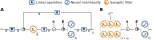
\includegraphics{media/chapters/02_modelling/02_03/nef_dynamics_diagram_c.pdf}%
	{\phantomsubcaption\label{fig:nef_dynamics_neurons_a}}%
	{\phantomsubcaption\label{fig:nef_dynamics_neurons_b}}%
	\caption[Synaptic filters and LTI systems in NEF networks]{Synaptic filters and \LTI systems in \NEF networks.
	\textbf{(A)} \NEF realisation of an \LTI system. Homogeneous synaptic filters are modelled as $d$ filters placed before the encoder.
	\textbf{(B)} Technically, each of the $n \times m$ synaptic connections between a pre- and a post-population has its own synaptic filter. When scaled appropriately, the resulting filter matrix replaces the synaptic weights; however, this has drastically higher computational costs than placing $d$ filters ahead of the encoder.}
	\label{fig:nef_dynamics_neurons}
\end{figure}

Using the representation and transformation principles, we can turn the block-diagram in \Cref{fig:nef_dynamics_synaptic} into a spiking neural network.
This is schematically depicted in \Cref{fig:nef_dynamics_neurons_a}.
The decoded state $\vec{\hat x}$ and the input $\vec u$ are passed through compensated \LTI matrices $\mat A'$ and $\mat B'$, summed, and fed into the synaptic filters.
We provided an example of this in \Cref{fig:nef_overview}.

Of course, as before, the network can, due to linearity, be expanded into biologically plausible synaptic weights and arrays of synaptic filters (\Cref{fig:nef_dynamics_neurons_b}).
Function decoders $\mat D^f$ can be used to support arbitrary nonlinear dynamics, and not just \LTI systems.

\subsection{Some Limitations of the Neural Engineering Framework}
\label{sec:nef_limitations}

To date, the Neural Engineering Framework has seen considerable use in the scientific community (cf.~\Cref{app:nef_literature}).
Nevertheless, the \NEF has a series of shortcomings that limit the biological plausibility of the generated networks, the number of constraints exposed to modellers, and how well resources available on some neuromorphic hardware platforms are utilised.
Resolving these issues could make the \NEF more appealing to a wider group of researchers and contribute to ongoing efforts in cognitive science and neuromorphic computing.

Of course, the following list of limitations is by no means complete.
To the contrary.
One can quite effortlessly identify areas of neuroscience that are not reflected in the \NEF at all---for example nervous system development, or networks of glial cells.
However, as we implied in the beginning this chapter, we think that, as of now, there is too little consensus on these topics to account for them in a general-purpose modelling tool.

Overall, while it is tempting to incorporate as much biological detail as possible into \NEF networks, this is misguided if merely done as an end in itself.
Remember that our goal is to bridge low-level mechanism and high-level function.
This distinguishes \NEF models from \enquote{bottom-up} approaches, that develop mechanistically detailed models of brain circuits, with the hope that the final system---if truthfully describing biology---exhibits some interesting function \citep[cf.][]{komer2016unified}.
We think that, optimally, extensions to the \NEF should expose new low-level detail as a \enquote{computational resource} that can be systematically exploited for high-level function.
At the very least, extensions should expose additional constraints that provide modellers with an opportunity to explore the impact of individual aspects of neurobiological mechanism on high-level function \citep[e.g.,][]{duggins2017incorporating}.
% TODO: Cite Pete's paper when published

%The two main extensions to the NEF we discuss in this thesis---nonlinear dendritic interactions and temporal tuning---fall into the first category, whereas the other extensions provide additional modelling constraints.

\subsubsection{Limitation 1: Current-based synapses}
In our discussion of Principle 2 (\Cref{sec:nef_transformation}), we implicitly assumed that neurons use current-based synapses (cf.~\Cref{sec:simplified_neuron_models}).
As expressed in \cref{eqn:nef_weight_vector}, we model the current injected into the post-neuron as linearly depending on the pre-population activities.
However, as we discussed in \Cref{sec:synaptic_transmission}, synaptic transmission is better modelled in terms of \emph{conductances}, and not currents.
As noted by \citet[Section~2.1.2, p.~35]{eliasmith2003neural}, accounting for conductances adds another layer of nonlinearity to the neuron.
While such nonlinearities have been analysed in the context of the \NEF by \citet[Chapter~4]{tripp2009search} as well as \citet{bobier2014unifying}, this prior work does not propose a systematic method for exploiting synaptic nonlinearities for computation.

Adapting the \NEF to support nonlinear conductance-based synapses would increase compatibility with neuromorphic hardware platforms emulating conductance-based neurons (e.g.,~BrainScaleS; \cite{schemmel2010waferscale}) and allow modellers to more easily constrain models according to neurophysiological parameters, such as synaptic reversal potentials.
Furthermore, individual synapse types (e.g.,~excitatory and inhibitory) act as independent input channels to a neuron.
As we discuss in the next chapter, these input channels interact nonlinearly in the case of multi-compartment neurons, increasing the class of functions that can be approximated using the same number of neurons.


\subsubsection{Limitation 2: Bias currents}
A minor (as we will see) limitation is the assumption that each neuron possess an intrinsic bias current $\beta_i$ (eq.~\ref{eqn:encoding}).
This current is necessary to ensure diverse tuning.
For example, some neurons are active even if no input is present (\enquote{spontaneous} or \enquote{background} activity).
This can be modelled using positive bias currents.

\Citet[Chapter~2; p.~35]{eliasmith2003neural} interpret the bias current as a \enquote{constant input current from the rest of the nervous system}.
While reasonable, this assumption cannot be strictly true.
The mean firing rate of individual populations varies sigificantly over time \citep{okun2012population}; it is not immediately clear how these variations would support constant $\beta_i$.
Hence, an explicit translation of pre-activities into a bias current $\beta_i$ using synaptic connectivity may be preferable.
Depending on the pre-population tuning, this can affect high-level function.


\begin{figure}
	\includegraphics{media/chapters/02_modelling/02_03/granule_jbias_distribution.pdf}%
	{\phantomsubcaption\label{fig:jbias_a}}%
	{\phantomsubcaption\label{fig:jbias_b}}%
	{\phantomsubcaption\label{fig:jbias_c}}%
	{\phantomsubcaption\label{fig:jbias_d}}%
	{\phantomsubcaption\label{fig:jbias_e}}%
	{\phantomsubcaption\label{fig:jbias_f}}
	\caption[Neuron parameter variability only accounts for small bias currents]{Neuron parameter variability only accounts for small bias currents.
	\textbf{(A, B)} Standard \NEF tuning curves and corresponding bias current distribution.
	\textbf{(C)} Empirical data on resting potential $v_\mathrm{rest}$ variations in cerebellar granule cells from \citet[Figure~1b]{chadderton2004integration} with a Gaussian fit.
	\textbf{(D)} Noisy \LIF neuron response curves for resting potentials samples from the empirical distribution. Colours indicated in \emph{(C)}. Other \LIF parameters fit to empirical data at $v_\mathrm{rest} = \SI{-64}{\milli\volt}$ (black crosses; cf.~Figure~1g in Chadderton et al.). Input currents $J$ are subject to Gaussian noise ($\sigma = \SI{10}{\pico\ampere}$). \textbf{(E)} Histogram of bias currents $\beta_i$ having the same average effect as varying $v_\mathrm{rest}$.
	\textbf{(F)}~Tuning curves that can be realised using these bias currents for the target maximum rates.
	Unfortunately, the empirically observed parameters do not result in tuning curve distributions assumed by the \NEF \emph{(A)}.}
	\label{fig:granule_jbias_distribution}
	\vspace*{-0.5em}
\end{figure}

Furthermore, and directly related to Limitation~1, pre-synaptic activity affects synaptic \emph{conductances} and does not directly induce \emph{currents}.
This is particularly problematic since tuning curves with uniform $x$-intercepts tend to require large \emph{negative} bias currents (\Cref{fig:jbias_a,fig:jbias_b}).
It is unclear how such currents should be generated, particularly since the inhibitory synaptic reversal potential $E_\mathrm{I}$ is close to the resting potential $v_\mathrm{rest}$.
Natural neuron parameter variations are insufficient to explain this discrepancy (\Cref{fig:jbias_c,fig:jbias_d,fig:jbias_e,fig:jbias_f}).

\begin{figure}
	\includegraphics{media/chapters/02_modelling/02_03/constrained_weight_matrices.pdf}
	{\phantomsubcaption\label{fig:sparsity_and_dales_principle_a}}%
	{\phantomsubcaption\label{fig:sparsity_and_dales_principle_b}}%
	{\phantomsubcaption\label{fig:sparsity_and_dales_principle_c}}%
	\caption[Constrained connectivity and Dale's principle]{Constrained connectivity and Dale's principle. \emph{Top:} Weight matrix $\mat W$ and (if applicable) factorisation into $\mat E, \mat D$. \emph{Bottom:} Weight histogram relative to the $95$-percentile $P_{95}$. Red indicates inhibitory, blue to excitatory weights. \textbf{(A)}~Typical \NEF weight matrices are dense.
	\textbf{(B)}~$L_1$-regularisation of decoders $\mat D$ increases sparseness, but does so in an uncontrolled manner. Note that $\mat D$ is (relatively speaking) sparser than $\mat W$.
	\textbf{(C)}~Dale's principle imposes an excitatory/inhibitory split on $\mat W$.
	This is difficult when factorising $\mat W$, but one can solve for $\mat W$ directly using nonnegative least-squares (\NNLS).
	}
	\label{fig:sparsity_and_dales_principle}
\end{figure}

\subsubsection{Limitation 3: Constrained connectivity and Dale's principle}
\NEF weight matrices $\mat W = \mat E \mat D$ are typically dense.
That is, they contain few zeros, implying all-to-all connectivity between neurons (\Cref{fig:sparsity_and_dales_principle_a}).
However, in biology, connectivity in the brain can be quite sparse.
For example, as detailed by \citet[Chapter~20]{braitenberg1998cortex}, the likelihood of two neighbouring cortical cells to be connected is less than $90\%$. Similarly, connectivity between Golgi and Granule cells in the cerebellum is highly constrained (cf.~Chapter~5).
% TODO: Add reference to Chapter 5
It may be desirable to give modellers the opportunity to account for these statistics.

A common way to enforce sparsity is to use $L_1$, or \enquote{lasso}, regularisation instead of the $L_2$ regularisation proposed in \cref{eqn:lstsq_loss_identity,eqn:lstsq_loss_f} \citep[Chapter~6]{boyd2004convex}.
However, solving for sparse decoders $\mat D$ in this way has two issues.
First, this process is uncontrolled---na\"ive $L_1$ regularisation does not take biological constraints into account.
Second, for $\Ndim \gg 1$, orthogonality between the encoders and decoders determines sparsity, and not just the sparsity of $\mat D$ (\Cref{fig:sparsity_and_dales_principle_b}).
Both issues mandate more complex regularisation terms.

Another form of constrained connectivity is to account for Dale's principle.
As we discussed before in \Cref{sec:synaptic_transmission}, individual neurons typically act either exclusively excitatorily or inhibitorily. Empirical data suggest that, depending on the modeled brain region, excitatory cells outnumber inhibitory cells by a factor between two and four~\citep{hendry1981sizes,gabbott1986quantitative}.
This imposes a certain structure onto the weight matrix (\Cref{fig:sparsity_and_dales_principle_c}).

\begin{figure}
	\centering
	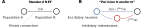
\includegraphics{media/chapters/02_modelling/02_03/parisien_transform.pdf}
	\caption[Illustration of the \enquote{Parisien transform}]{Illustration of the \enquote{Parisien transform}. This transformation accounts for Dale's principle by splitting standard \NEF connections, as depicted in \textbf{(A)}, into an excitatory and inhibitory path \textbf{(B)}.}
	\label{fig:parisien_transform}
\end{figure}

\Citet[Section~6.4]{eliasmith2003neural} propose a method to account for Dale's principle later refined by \citet{parisien2008solving}.
The basic idea of this \enquote{Parisien transform} is to add a specially crafted \enquote{bias function} to the function computed in the excitatory connection.
This bias function ensures that all connection weights are positive.
An inhibitory inter-neuron population is then added to the network and connected in parallel to the excitatory connection to subtract the superfluous current induced by the bias function (\Cref{fig:parisien_transform}).

While mathematically clever, the Parisien transform changes the network structure by adding an inhibitory interneuron population.
Although interneurons are indeed common in brain networks, the connectivity patterns resulting from the Parisien transform may not be desirable.
For example, as we discuss in Chapter~5, Golgi cells are recurrent inhibitory interneurons between granule cells.
However, there are no excitatory recurrent connections between granule cells, as assumed by the Parisien transform.
In the next chapter, we discuss an approach to accounting for Dale's principle that is independent of the network structure.

\subsubsection{Limitation~4: Temporal tuning and neural dynamics}
The dynamics principle derived in \Cref{sec:nef_dynamics} was based on two assumptions.
First, synaptic dynamics dominate neural dynamics.
Second, synaptic filters are homogeneous first-order low-pass filters in both the input and recurrent connection.
While reasonable, these modelling assumptions are, as so often, only coarse approximations of biology.

\begin{figure}[t]
	\includegraphics{media/chapters/02_modelling/02_03/firing_rate_neural_dynamics.pdf}
	\caption[Neural dynamics for different maximum firing rates]{Neural dynamics for different maximum firing rates $a_\mathrm{max}$. A \SI{100}{\second} band-limited white-noise signal $u(t)$ with a band-width of \SI{100}{\hertz} is fed through an \NEF population with uniform $x$-intercepts.
	The transfer function is determined from the decoded $\hat u(t)$ using the method described in \citet[Section~4.3.3]{eliasmith2003neural}.
	We ensure a constant amount of spike noise by setting the number of neurons in the population to $100\,000 / a_\mathrm{max}$. \emph{Top:} Linear transfer function for different maximum rates $a_\mathrm{max}$. \emph{Bottom:} Slice through the transfer functions at the indicated locations.
	\textbf{(A)} Data for a spiking rectified linear unit (\ReLU), a $\Delta\Sigma$-modulator with a rectified input current. This kind of neuron exhibits no significant dynamics of its own, independent of the firing rate. \textbf{(B)} Transfer function for the \LIF neuron. For small firing rates, the neuron acts as a low-pass with a relatively moderate attenuation of about \SI{-5}{\deci\bel}. For firing rates of about \SI{200}{\hertz}, the neuron acts as a pass-through. \textbf{(C)} While similar to the \LIF neuron, the \ALIF
	acts as a very narrow low-pass filter when driven at a maximum firing rate of about \SI{20}{\hertz}. The location of this \enquote{trough} depends on the adaptation time-constant.}
	\label{fig:neural_dynamics_firing_rates}
\end{figure}

The assumption that synaptic dynamics dominate the overall dynamics of a neuron is a good approximation of the behaviour of simple neuron models operating at high firing-rates.
However, for smaller firing rates, the neural dynamics can have a significant impact on the overall system dynamics.
For example, for maximum firing rates below about $\SI{50}{\per\second}$, the sub-threshold low-pass dynamics of the \LIF neuron begin to have a moderate effect on the neural dynamics.
This is depicted in \Cref{fig:neural_dynamics_firing_rates}.

While these rate-dependent effects are relatively small, more complex neuron models possess strong intrinsic dynamics.
For example, the adaptive \LIF (\ALIF) neuron model \citep{camera2004minimal} accounts for firing rate adaptation; that is, each output spike increases the current required to evoke another output spike.
This can be modelled as an inhibitory current resulting from low-pass filtering the neuron's output spike train.
As demonstrated by \citet[Chapter~7]{tripp2009search}, the internal dynamics of the \ALIF neuron model can, under certain circumstances, be exploited to implement arbitrary dynamics using a variant of the equations derived for the \NEF dynamics principle.

The second assumption, namely that synaptic filters are homogeneous, is likely violated if a neuron possesses multiple receptor types.
As we saw in \Cref{sec:synaptic_transmission}, the synaptic time-constant can vary significantly between (and even within) individual receptor types.
We also saw that synaptic transmission is better modelled by higher-order filters.
\Citet{voelker2018improving} discuss methods to generalise the dynamics principle to arbitrary synaptic filters; however, these methods require access to the input signal differentials.

In \Cref{chp:temporal_tuning}, we suggest the concept of \enquote{temporal tuning curves} to---at least partially---account for these issues.
Temporal tuning curves are a direct extension of standard \NEF tuning curves, and are inspired by the concept of temporal receptive fields.
In essence, we treat both synaptic and neural dynamics as temporal resources that can be harnessed to approximate a desired temporal tuning by solving a simple least-squares problem.
This naturally extends the \NEF and, to an extent, unifies the approaches described by Tripp and Voelker systematically.
